%%%%%%%%%%%%%%%%%%%%%%%%%%%%%%%%%%%%%%%%%%%%%%%%%%%%%%%%%%%%%%%%%%%%%%%%%%%%%%%%%%%%%%%%%%%%%%%%%%%%%%%%%%%%%%%%%%%%%%%%%%%%%%%%%%%%%%%%%%%%%%%%%%%%%%%%%%%
% This is just an example/guide for you to refer to when submitting manuscripts to Frontiers, it is not mandatory to use Frontiers .cls files nor frontiers.tex  %
% This will only generate the Manuscript, the final article will be typeset by Frontiers after acceptance.
%                                              %
%                                                                                                                                                         %
% When submitting your files, remember to upload this *tex file, the pdf generated with it, the *bib file (if bibliography is not within the *tex) and all the figures.
%%%%%%%%%%%%%%%%%%%%%%%%%%%%%%%%%%%%%%%%%%%%%%%%%%%%%%%%%%%%%%%%%%%%%%%%%%%%%%%%%%%%%%%%%%%%%%%%%%%%%%%%%%%%%%%%%%%%%%%%%%%%%%%%%%%%%%%%%%%%%%%%%%%%%%%%%%%

%%% Version 3.4 Generated 2018/06/15 %%%
%%% You will need to have the following packages installed: datetime, fmtcount, etoolbox, fcprefix, which are normally inlcuded in WinEdt. %%%
%%% In http://www.ctan.org/ you can find the packages and how to install them, if necessary. %%%

\documentclass[utf8]{frontiers/frontiersSCNS}

%\setcitestyle{square} % for Physics and Applied Mathematics and Statistics articles
\usepackage{url,hyperref,lineno,microtype,subcaption}
\usepackage[onehalfspacing]{setspace}

\linenumbers


% BELOW TAKEN FROM rticles plos template
%
% amsmath package, useful for mathematical formulas
\usepackage{amsmath}
% amssymb package, useful for mathematical symbols
\usepackage{amssymb}

% hyperref package, useful for hyperlinks
\usepackage{hyperref}

% graphicx package, useful for including eps and pdf graphics
% include graphics with the command \includegraphics
\usepackage{graphicx}

% Sweave(-like)
\usepackage{fancyvrb}
\DefineVerbatimEnvironment{Sinput}{Verbatim}{fontshape=sl}
\DefineVerbatimEnvironment{Soutput}{Verbatim}{}
\DefineVerbatimEnvironment{Scode}{Verbatim}{fontshape=sl}
\newenvironment{Schunk}{}{}
\DefineVerbatimEnvironment{Code}{Verbatim}{}
\DefineVerbatimEnvironment{CodeInput}{Verbatim}{fontshape=sl}
\DefineVerbatimEnvironment{CodeOutput}{Verbatim}{}
\newenvironment{CodeChunk}{}{}

% cite package, to clean up citations in the main text. Do not remove.
\usepackage{cite}

\usepackage{color}

% Below is from frontiers
%
\bibliographystyle{frontiersinSCNS}
% Use doublespacing - comment out for single spacing
%\usepackage{setspace}
%\doublespacing


% Leave a blank line between paragraphs instead of using \\


\def\keyFont{\fontsize{8}{11}\helveticabold }


%% ** EDIT HERE **
%% PLEASE INCLUDE ALL MACROS BELOW

%% END MACROS SECTION


% tightlist command for lists without linebreak
\providecommand{\tightlist}{%
  \setlength{\itemsep}{0pt}\setlength{\parskip}{0pt}}

% From pandoc table feature
\usepackage{longtable,booktabs,array}
\usepackage{calc} % for calculating minipage widths
% Correct order of tables after \paragraph or \subparagraph
\usepackage{etoolbox}
\makeatletter
\patchcmd\longtable{\par}{\if@noskipsec\mbox{}\fi\par}{}{}
\makeatother
% Allow footnotes in longtable head/foot
\IfFileExists{footnotehyper.sty}{\usepackage{footnotehyper}}{\usepackage{footnote}}
\makesavenoteenv{longtable}

% Pandoc citation processing
\newlength{\cslhangindent}
\setlength{\cslhangindent}{1.5em}
\newlength{\csllabelwidth}
\setlength{\csllabelwidth}{3em}
\newlength{\cslentryspacingunit} % times entry-spacing
\setlength{\cslentryspacingunit}{\parskip}
% for Pandoc 2.8 to 2.10.1
\newenvironment{cslreferences}%
  {}%
  {\par}
% For Pandoc 2.11+
\newenvironment{CSLReferences}[2] % #1 hanging-ident, #2 entry spacing
 {% don't indent paragraphs
  \setlength{\parindent}{0pt}
  % turn on hanging indent if param 1 is 1
  \ifodd #1
  \let\oldpar\par
  \def\par{\hangindent=\cslhangindent\oldpar}
  \fi
  % set entry spacing
  \setlength{\parskip}{#2\cslentryspacingunit}
 }%
 {}
\usepackage{calc}
\newcommand{\CSLBlock}[1]{#1\hfill\break}
\newcommand{\CSLLeftMargin}[1]{\parbox[t]{\csllabelwidth}{#1}}
\newcommand{\CSLRightInline}[1]{\parbox[t]{\linewidth - \csllabelwidth}{#1}\break}
\newcommand{\CSLIndent}[1]{\hspace{\cslhangindent}#1}

\usepackage{float}

\def\Authors{
  Bjørn Peare Bartholdy\,\textsuperscript{1*},
  Amanda G. Henry\,\textsuperscript{1}}

\def\Address{

  \textsuperscript{1} Archaeological Sciences, Leiden University,  Leiden,   Netherlands
  }

  \def\corrAuthor{Bjørn Peare Bartholdy}\def\corrAddress{Leiden University\\Einsteinweg 2\\Leiden, 2333 CC Netherlands}\def\corrEmail{\href{mailto:b.p.bartholdy@arch.leidenuniv.nl}{\nolinkurl{b.p.bartholdy@arch.leidenuniv.nl}}}
  \def\firstAuthorLast{BARTHOLDY {et~al.}}
  
  


\begin{document}

\onecolumn
\firstpage{1}


\title[Biases Associated with Starch Incorporation]{Investigating Biases Associated with Dietary Starch Incorporation and Retention with an Oral Biofilm Model}
\author[\firstAuthorLast]{\Authors}
\address{} %This field will be automatically populated
\correspondance{} %This field will be automatically populated

\extraAuth{}% If there are more than 1 corresponding author, comment this line and uncomment the next one.
%\extraAuth{corresponding Author2 \\ Laboratory X2, Institute X2, Department X2, Organization X2, Street X2, City X2 , State XX2 (only USA, Canada and Australia), Zip Code2, X2 Country X2, email2@uni2.edu}


\maketitle

\begin{abstract}



Dental calculus has proven to contain a wealth of information on the
dietary habits of past populations. These insights have, to a large
extent, been obtained by the extraction and identification of starch
granules contained within the mineralised dental plaque from a wide
range of regions and time periods. The scope of previous studies have
been limited to microfossil extraction and identification to reconstruct
dietary preferences from the archaeological record, and few studies have
attempted to address the biases of starch retention in dental calculus.
Those that have considered this problem have been limited to \emph{in
vivo} studies on modern humans and non-human primates. Here, we present
a multispecies oral biofilm model, which allows experimental research on
starch incorporation and retention to be conducted on \emph{in vitro}
dental calculus in a controlled laboratory setting. The biofilms were
exposed to treatment solutions with known quantities of dietary starches
(wheat and potato) during the 25-day growth period. After this, the
starch granules were extracted from the mature biofilm (by dissolution
in EDTA), and counted. We show that the granule counts extracted from
the model dental calculus represented a low proportion (ranging from
0.06\% to 0.16\%) of the total number of granules exposed to the
biofilms throughout the experiment. Additionally, we found that the
ratios of granule sizes from the extracted starch granules differed from
the original treatment solutions, with large granules (\textgreater20
\(\mu\)m) consistently being under-represented. We also found a
positive correlation between the absolute granule counts and dry-weight of the
biofilm (\emph{r} = 0.659, 90\%CI{[}0.463, 0.794{]}), meaning the absolute
quantity of starch granules will increase as the size of the calculus deposit
increases. A similar, but weaker correlation was found between
the concentration (count per mg) of granules and dry-weight (\emph{r} =
0.3, 90\%CI{[}0.0618, 0.506{]}).\\
Our results complement and reinforce previous \emph{in vivo} studies suggesting
that dental calculus presents a very small, and partly biased picture of the
original dietary intake of starches, with an over-representation of
plants producing granules smaller than 20 \(\mu\)m in size. The
experimental model presented here is well-suited to address the need for
further validation of methods and biases associated with dietary
research on dental calculus.


\tiny
 \keyFont{ \section{Keywords:} oral biofilm model, starch, alpha-amylase, dental calculus, paleodiet reconstruction}
 
\end{abstract}

\hypertarget{introduction}{%
\section{Introduction}\label{introduction}}

Dental calculus has proven to contain a wealth of
dietary information in the form of plant microfossils
(Henry and Piperno, 2008; Hardy et al., 2009),
proteins (Hendy et al., 2018; Warinner et al., 2014a),
and other organic residues (Buckley et al., 2014).
This dietary information can be preserved within the mineralised dental plaque
over many millennia, providing a unique window into the food-related behaviours of
past populations
(Henry and Piperno, 2008; Jovanović et al., 2021; Tao et al., 2020)
and extinct species (Henry et al., 2014; Hardy et al., 2012).

Until recently, only a few studies directly investigated the presence of plant
microremains
in the dental calculus of archaeological remains. The ability to extract phytoliths
from the dental calculus of archaeological fauna to investigate diet was first
noted by Armitage (1975),
and later by Middleton and Rovner (1994),
and Fox and colleagues (1996). Starches and phytoliths were
extracted from human dental calculus by Cummings and Magennis (1997).\\
In more recent years, the study of dental calculus has increased exponentially,
and the wealth of information contained within the mineralised matrix has largely
been acknowledged. The use of dental calculus spans a wide
variety of archaeological research areas, such as oral microbiome
characterisation (including pathogens) through the analysis of DNA and proteins
(Adler et al., 2013; Warinner et al., 2014b),
microbotanical remains (Henry and Piperno, 2008; Hardy et al., 2009; Mickleburgh and Pagán-Jiménez, 2012),
other organic residues and proteins from dietary compounds
(Buckley et al., 2014; Hendy et al., 2018),
and nicotine use (Eerkens et al., 2018). Especially the extraction
of starch granules has become a rich source of dietary
information, as starch granules have proven to preserve well within dental calculus
over a variety of geographical and temporal ranges
(Piperno and Dillehay, 2008; Henry et al., 2014; Tao et al., 2020; Jovanović et al., 2021).

Despite this, our knowledge of dental calculus and the incorporation pathways of
the various markers is limited (Radini et al., 2017), as is our
knowledge of information-loss caused by these pathways. Additionally, the methods
we use to extract and analyse dental calculus, and make inferences on past diets
represent another potential source of bias. Studies on both archaeological and
modern individuals have explored these biases in more detail.
Extraction methods were tested
by Tromp and colleagues (2017), specifically regarding
decalcification using HCl or EDTA.
The authors found significantly more starches with the EDTA extraction method
than the HCl extraction method; however, as noted by the authors, comparisons
involving archaeological calculus are problematic due to variability between and
within individuals.
Studies conducted on modern humans (Leonard et al., 2015)
and non-human primates (Power et al., 2015; Power et al., 2021)
have explored how well microremains (phytoliths and starches)
extracted from dental calculus represent the actual dietary intake.
These studies are justifiably limited,
despite meticulous documentation and observation, due to unknown variables and
uncertainty involved in this kind of \emph{in vivo} research. Dental calculus is a complex
oral biofilm with a multifactorial aetiology and variable formation rates both
within and between individuals (Jepsen et al., 2011; Haffajee et al., 2009),
contributing to
the stochasticity of starch representation being observed in numerous studies.
Additionally, the concentration of oral \(\alpha\)-amylase differs both between and
within individuals (Froehlich et al., 1987; Nater et al., 2005),
causing different rates of hydrolysis of the starch granules present in the oral
cavity. Add to this the effects of the many different methods
of starch processing (Hardy et al., 2018), as well as post-depositional
processes that are still being explored
(García-Granero, 2020; Mercader et al., 2018),
and it becomes clear that using
dental calculus to reconstruct diet is a highly unpredictable process.

In this exploratory study, we use an oral biofilm model to investigate the
retention of starch granules within dental calculus in a controlled laboratory
setting, allowing us full control over dietary input. Our main questions concern
the representation of granules extracted
from the calculus compared to the actual intake. How much of the original diet is
incorporated into the calculus, and how much is recovered?
Is there differential loss of information from specific dietary markers that affects
the obtained dietary information, and how does this affect the representation of
diet from extracted microremains?\\
We find that, despite the absence of \(\alpha\)-amylase in
the model, a limited proportion of the starch input is actually
retained in the calculus. We also observed a shift in the size ratios of individual
starch granules that are incorporated into the calculus, and that the number of
incorporated starch granules increases as the size of the calculus deposit
increases.

\hypertarget{materials-and-methods}{%
\section{Materials and Methods}\label{materials-and-methods}}

\hypertarget{biofilm-formation}{%
\subsection{Biofilm formation}\label{biofilm-formation}}

In this study we employ a multispecies oral biofilm model following a modified
protocol from Sissons and colleagues (1991) and
Shellis (1978). In brief, a biofilm inoculated
with whole saliva was grown on a substrate suspended in artificial saliva, and
fed with sugar (sucrose). After several days of growth, the biofilm was exposed
to starch solutions. Mineralisation of the biofilm was aided by exposure to a
calcium phosphate solution. After 25 days of growth, the mineralised biofilm was
collected for further analysis. The setup comprises a polypropylene
24 deepwell PCR plate (KingFisher 97003510) with a lid containing 24 pegs, which
is autoclaved at 120°C, 1 bar overpressure, for 20 mins. The individual pegs
were the substrata on which the calculus grew. Using this system allowed for easy
transfer of the growing biofilm between saliva, feeding solutions,
and mineral solutions.

The artificial saliva (AS) is a modified version of the basal medium mucin (BMM)
described by Sissons and colleagues (1991).
It contains 2.5 g/l partially purified mucin from porcine stomach (Type III, Sigma M1778),
5 g/l trypticase peptone (Roth 2363.1), 10 g/l proteose peptone (Oxoid LP0085),
5 g/l yeast extract (BD 211921), 2.5 g/l KCl, 0.35 g/l NaCl, 1.8 mmol/l CaCl\textsubscript{2},
5.2 mmol/l Na\textsubscript{2}HPO\textsubscript{4} (Sissons et al., 1991), 6.4 mmol/l NaHCO\textsubscript{3}
(Shellis, 1978), 2.5 mg/l haemin. This is subsequently
adjusted to pH 7 with NaOH pellets and stirring, autoclaved (15 min, 120°C,
1 bar overpressure), and supplemented with 5.8 \(\mu\)mol/l menadione, 5 mmol/l urea,
and 1 mmol/l arginine (Sissons et al., 1991).

Fresh whole saliva (WS) for inoculation was provided by a 31-year-old male donor
with no history of caries, who abstained from oral hygiene for 24 hours. No
food was consumed two hours prior to donation and no antibiotics were taken up
to six months prior to donation.
The saliva was filtered through a sterilised (with sodium hypochlorite, 10--15\% active chlorine)
nylon cloth to remove particulates.
Substrata were inoculated with 1 ml/well of a two-fold dilution of WS in sterilised
20\% (v/v) glycerine for four hours at 36°C, to allow attachment of the
salivary pellicle and plaque-forming bacteria. After initial inoculation, the
substrata were transferred to a new plate containing 1 ml/well AS and incubated
in a shaking incubator (Infors HT Ecotron) at 36°C, 30 rpm.
The inoculation process was repeated on days 3 and 5.
AS was partially refreshed once per day and fully refreshed every three days,
throughout the experiment, by transferring the substrata to a new plate containing
stock AS. To feed the bacteria, the substrata were transferred to a new plate, containing
5\% (w/v) sucrose, for six minutes twice daily, except on inoculation days
(days 0, 3, and 5), where the samples only received one sucrose treatment after
inoculation.

Starch treatments were initiated on day 9 to avoid starch granule counts being
affected by \(\alpha\)-amylase hydrolysis from saliva inoculation days.
An \(\alpha\)-amylase (EC 3.2.1.1) activity
assay was conducted to confirm that no amylase was present in the model before
starch treatments started. Starch treatments replaced sucrose treatments, occurring twice per day
for six minutes. The starch treatments involved transferring the substrata to a
new plate containing a 0.25\% (w/v) starch from potato (Roth 9441.1) solution, a 0.25\% (w/v) starch from wheat (Sigma S5127) solution, and a 0.5\% (w/v) mixture of equal
concentrations (w/v) wheat and potato. All starch treatments were created in dH\textsubscript{2}O
with 5\% (w/v) sucrose. Before transferring biofilm samples to the starch treatment
plate, the plates were agitated to keep the starches in suspension in the
solutions. During treatments, the rpm was increased to 60 to facilitate contact
between starch granules and biofilms.

After 15 days, mineralisation was encouraged with a
calcium phosphate monofluorophosphate urea (CPMU) solution containing
20 mmol/l CaCl\textsubscript{2}, 12 mmol/l NaH\textsubscript{2}PO\textsubscript{4}, 5 mmol/l Na\textsubscript{2}PO\textsubscript{3}F, 500 mmol/l urea,
and (0.04 g/l MgCl)
(Pearce and Sissons, 1987; Sissons et al., 1991).
The substrata were submerged in 1 ml/well CPMU for six minutes, five times
daily, in a two-hour cycle. During the mineralisation period, starch treatments
were reduced to once per day after the five CPMU treatments. This process was repeated
for 10 days until the end of the experiment on day 24
(see Figure \ref{fig:protocol-fig} for an overview of the protocol).

All laboratory work was conducted in sterile conditions under a laminar flow hood
to prevent starch and bacterial contamination. Control samples that only received
sucrose as a treatment were included to detect starch contamination from the
environment or cross-contamination from other wells in the same plate.

\hypertarget{amylase-activity-detection}{%
\subsection{Amylase activity detection}\label{amylase-activity-detection}}

An \(\alpha\)-amylase (EC 3.2.1.1) activity assay was conducted on artificial
saliva samples collected from the plate wells on days 3, 6, 8, 9, 10, 12, and 14.
Whole saliva samples were collected on days 0, 3, and 5 as positive controls.
Collected samples were stored at 4°C until the assay was conducted on day 18.
All samples and standard curves were run in triplicates on two separate plates.
Positive control saliva samples were compared against a standard curve containing
H\textsubscript{2}O, while artificial saliva samples were compared against a standard curve
containing stock AS (due to the colour of artificial saliva).
Two photometric readings were conducted for each plate with a 540 nm filter on a
Multiskan FC Microplate Photometer (Thermo Scientific 51119000).
The protocol is a modified version of an Enzymatic Assay of \(\alpha\)-Amylase
(\url{https://www.sigmaaldrich.com/NL/en/technical-documents/protocol/protein-biology/enzyme-activity-assays/enzymatic-assay-of-a-amylase}) (Bernfeld, 1955), which measures the amount of
maltose released from starch by \(\alpha\)-amylase activity. Results are reported
in units (U) per mL enzyme, where 1 U releases 1 \(\mu\)mole of maltose in 6 minutes.
The detailed protocol can be found here: \url{https://www.protocols.io/view/amylase-activity-bw8jphun}.

\hypertarget{treatment-solutions}{%
\subsection{Treatment solutions}\label{treatment-solutions}}

A 1 ml aliquot of each starch solution was taken, from which 10 \(\mu\)l was mounted
on a microscope slide with an 18 x 18 mm coverslip, and counted under a light microscope
(Zeiss Axioscope A1). For wheat and mixed treatment samples, we counted three
slide transects (at ca. 1/4, 1/2, and 3/4 of the slide), and the sample counts
were extrapolated to the total number of granules exposed to the samples over 16
days of treatments (see Supplementary Material for more details). For potato
treatment samples, the whole slide was counted.

\hypertarget{extraction-method}{%
\subsection{Extraction method}\label{extraction-method}}

Extraction of starches from the calculus samples was performed by dissolving the
calculus in 0.5 \(\tiny{M}\) ethylenediaminetetraacetic acid (EDTA)
(Tromp et al., 2017; Le Moyne and Crowther, 2021; Modi et al., 2020),
and vortexing for 3 days until the sample was completely dissolved.
Twenty \(\mu\)l of sample was mounted onto a slide with an 18x18 mm coverslip.
When transferring the sample to the slide, the sample was homogenised using
the pipette to ensure that the counted transects were representative of the
whole slide. The count from the slide was extrapolated to the whole sample
(see Supplementary Material for more detail).

Both wheat and potato granules were divided into three size categories:
small (\textless10 \(\mu\)m), medium (10 -- 20 \(\mu\)m), and large (\textgreater20 \(\mu\)m).

\hypertarget{statistical-analysis}{%
\subsection{Statistical analysis}\label{statistical-analysis}}

Statistical analysis was conducted in R version 4.2.0 (2022-04-22) (R Core Team, 2020) and
the following packages: tidyverse (Wickham et al., 2019), broom (Robinson et al., 2021),
here (Müller, 2020), and patchwork (Pedersen, 2020).

To see if biofilm growth was differently affected by starch treatments, a
one-way ANOVA with sample weight as the dependent variable (DV) and treatment
as the grouping variable (GV) was conducted.
To analyse granule counts and calculate size proportions, mean counts for each
treatment were taken across
both experimental plates, resulting in a mean count for each
granule size category within each treatment.

Pearson's \emph{r} was conducted on sample weight and total starch count, as well as sample
weight and starch count per mg calculus. The total count for each sample within a
treatment was standardised by z-score to account for the differences in magnitude
between the potato and wheat counts.
This was applied to total biofilm weight and starch count per mg
calculus (also z-score standardised) to account for differences in starch
concentration in the calculus (as per Wesolowski et al., 2010).

\hypertarget{results}{%
\section{Results}\label{results}}

All samples yielded sufficient biofilm growth and starch incorporation to be
included in the analysis (Figure \ref{fig:microscope-fig}), resulting in a total of 48 biofilm samples (two plates of 24),
45 of which were used for analysis (three samples were set aside for later
analysis).
Most control samples contained no starch granules, while some contained negligible
quantities (see Supplementary Material).

\hypertarget{no-amylase-activity-detected-in-the-model}{%
\subsection{No amylase activity detected in the model}\label{no-amylase-activity-detected-in-the-model}}

No \(\alpha\)-amylase activity was detected in any of the artificial
saliva samples from any of the days that were sampled. Only positive controls
(saliva)
contained amylase activity that could be detected in the assay, ranging from
9.93 to 30.2 U/mL enzyme
(full results can be found in the Supplementary Material).
The results are not comparable to other studies presenting \(\alpha\)-amylase activity
levels in humans, as the unit definition may differ;
however, they are sufficient to show that there is no activity in the model.

\hypertarget{treatment-type-had-minimal-effect-on-biofilm-growth}{%
\subsection{Treatment type had minimal effect on biofilm growth}\label{treatment-type-had-minimal-effect-on-biofilm-growth}}

A one-way ANOVA suggests that the type of starch used during the biofilm
growth period had a minimal effect on the growth of the biofilm
(expressed as total dry weight of the sample), F(3, 43)
= 1.16, p = 0.335.
A summary of sample weights is available in Table \ref{tab:anova-tbl}.

\hypertarget{starch-counts}{%
\subsection{Starch counts}\label{starch-counts}}

It was not possible to differentiate between potato and
wheat starches smaller than ca. 10 \(\mu\)m. These were counted as wheat,
as we assumed that the majority of the small granules were wheat. We make this
assumption based on the counts of small starches in the wheat-only and potato-only
solutions. Of the combined amount of small starches in these two solutions,
99.2\%
are from wheat.

The separate wheat and potato solutions were made with a 0.25\% (w/v) starch
concentration, while the mixed-starch solution was made with 0.25\% (w/v) of each
starch, with a total concentration of 0.50\% (w/v).
The mixed treatment had the highest absolute count of starch granules in solution (mean = \ensuremath{2.9\times 10^{7}}),
while the biofilms exposed to the wheat solution preserved the greatest number of
granules
(mean = \ensuremath{2.77\times 10^{4}}).
The potato treatment had the lowest absolute counts in both the solution
(\ensuremath{3.02\times 10^{6}})
and in the biofilm samples
(4850)
(Tables \ref{tab:solution-count-tbl} and \ref{tab:sample-count-tbl}).

\hypertarget{proportion-of-available-starches-incorporated-in-samples}{%
\subsubsection{Proportion of available starches incorporated in samples}\label{proportion-of-available-starches-incorporated-in-samples}}

The proportion of total starches from the solutions that were incorporated
into the samples ranged from
0.06\% to 0.16\%,
with potato granules being more readily incorporated than wheat in both the
separated- and mixed-treatment samples
(Table \ref{tab:sample-prop-tbl}).
There is an inverse relationship between the absolute starch count in the solutions
and the proportional incorporation of starches in the biofilm samples, i.e., potato
had the lowest absolute count in solutions, but the highest proportional
incorporation, and vice versa for the mixed treatment.

Wheat incorporation was most affected in the mixed-treatment samples, with only
0.06\% of the total available starches being incorporated into
the sample, compared to
0.16\%
in the separated wheat treatment.

\hypertarget{size-ratios-differ-between-solutions-and-samples}{%
\subsubsection{Size ratios differ between solutions and samples}\label{size-ratios-differ-between-solutions-and-samples}}

Overall, medium starch granules had a higher mean rate of incorporation
(0.171\%)
than small
(0.120\%)
and large
(0.066\%)
starch granules across all treatments, while large potato starches had the lowest
rate of incorporation across all treatments.

The difference in incorporation between the size categories resulted in a change
in size ratios between the original starch solutions and the extracted samples.
Large potato granules (\textgreater{} 20 \(\mu\)m) were most affected, with a
32.3\%
decrease in relative abundance in the potato-only treatment, and a
26.5\%
decrease in mixed treatments. Medium granules increased in relative abundance
across all samples, while small granules decreased in wheat treatments and
increased in potato treatments
(Figure \ref{fig:ratio-plots}).

\hypertarget{biofilm-weight-correlated-positively-with-extracted-starch-counts}{%
\subsubsection{Biofilm weight correlated positively with extracted starch counts}\label{biofilm-weight-correlated-positively-with-extracted-starch-counts}}

Pearson's \emph{r} suggests a
strong positive
correlation between the total weight of the biofilms and the total starch count
(standardised by z-score) extracted from the samples across treatments,
\emph{r} = 0.659,
90\%CI{[}0.463, 0.794{]},
p \textless{} 0.001
(Figure \ref{fig:cor-plot}A).

The same test was applied to total biofilm weight and starch count per mg
calculus (also standardised by z-score), resulting in a weak positive correlation,
\emph{r} = 0.3,
90\%CI{[}0.0618, 0.506{]},
p = 0.0403
(Figure \ref{fig:cor-plot}B).

\hypertarget{discussion}{%
\section{Discussion}\label{discussion}}

Here, we have provided a method for exploring the incorporation of dietary
starches into the mineral matrix of a dental calculus biofilm model. Our results show
that a very low proportion of the starches exposed to the biofilm during growth are
retained in the mineral matrix, and that the size of the starch granules
may affect the likelihood of incorporation. The proportions of starch granules
(of all sizes) present in the extracted samples were similar across all treatments
(0.06\% to 0.16\%),
despite large differences in absolute granule counts between wheat
(mean = 25,404,000)
and potato
(mean = 3,016,000)
solutions.\\
The absolute counts, however, differed more visibly between treatments and was
proportional with the total count of granules in the treatment solutions. Wheat
and mixed solutions had the highest absolute mean count of starch granules, and
also had the highest absolute mean count of starch granules extracted from the
dental calculus
(Tables \ref{tab:solution-count-tbl} and \ref{tab:sample-count-tbl}).
This suggests that the starches that are more frequently consumed will be present
in higher quantities in the dental calculus, at least prior to inhumation and
degradation in the burial environment.
Despite the low proportion of granules recovered from the model calculus
(0.06\% to 0.16\%),
the absolute counts were still substantially greater than counts recovered from
archaeological remains
(Tromp and Dudgeon, 2015; Tromp et al., 2017; Wesolowski et al., 2010), which could in part be due to the
lack of oral amylase activity in our model.
Previous research conducted on dental calculus from contemporary humans and non-human
primates suggest a high level of stochasticity involved in the retention of
starch granules in dental calculus, and that starch granules extracted from dental
calculus are underrepresented with regard
to actual starch intake, which is consistent with our findings (illustrated by high
standard deviations and low proportional incorporation).
Leonard and colleagues (2015) found individual
calculus samples to be a poor predictor of diet in a population, as many of the
consumed plants were missing from some individual samples, but were present in others.\\
Power and colleagues (2015)
presented similar findings in non-human primates, where phytoliths were more
representative of individual diets than starch granules.
The size bias is also consistent with the findings by Power and colleagues
(2015),
who found that plants producing starches 10--20 \(\mu\)m in
size were over-represented; however, the representation of granules larger than
20 \(\mu\)m in their study is unclear.

We have also shown that the size of the starch granules influences the likelihood
of incorporation into the calculus. Starch granules larger than 20 \(\mu\)m in
maximum length were underrepresented in the calculus samples compared to the original
starch solutions, an effect that was consistent across all three treatments. Medium
granules (10--20 \(\mu\)m) were often over-represented
(Table \ref{tab:sample-prop-tbl},
and
Figure \ref{fig:ratio-plots}).
Large potato granules were most affected, potentially because of the greater
size-range. They can reach up to 100 \(\mu\)m in maximum length, whereas wheat
granules generally only reach up to 35 \(\mu\)m
(Gismondi et al., 2019; Haslam, 2004; Seidemann, 1966, 174--176).
Granule morphology may also play a role. Large wheat granules
are lenticular and have a larger surface area compared
to volume, whereas large potato granules are ovoid and have a larger volume
compared to surface area
(van de Velde et al., 2002; Jane et al., 1994; Reichert, 1913, 364--365; Seidemann, 1966, 174--176).
Another potentially important factor
from our results is the size of the calculus deposit. We found a
strong positive correlation between size of biofilm deposit and
retained starch granules (Figure \ref{fig:cor-plot}A), meaning larger calculus
deposits contain a higher quantity of granules;
a result that contradicts findings from archaeological contexts
(Wesolowski et al., 2010; Dudgeon and Tromp, 2014).
When the concentration of starch granules
per mg calculus is considered, the correlation is weaker, but still present
(Figure \ref{fig:cor-plot}B).
While the larger deposits contain a higher absolute count, our findings also suggest
that they contain a slightly higher concentration of starches. This may also explain
the lower mean retention of starch granules in mixed treatments compared to
wheat treatments. Wheat treatment samples (mean = 5.53 mg) were on average larger than mixed treatment samples (mean = 4.28 mg) (Table \ref{tab:anova-tbl}); and while mixed treatment solutions contained the highest mean overall
granule counts, wheat treatment samples had the highest mean starch retention.
Further research is needed to determine why this differs from previous archaeological
findings.

The mechanism by which starch granules are incorporated into plaque and calculus
remains largely unknown, and few studies have directly investigated potential
mechanisms. We know that a proportion of the starch granules entering
the mouth can become trapped in the plaque/calculus, and can be recovered from
archaeological samples of considerable age
(Henry et al., 2014; Buckley et al., 2014; Wu et al., 2021).
Studies have also shown that not all starch granules come from a dietary source.
Other pathways include cross-contamination from plant interactions in soil, such
as palm phytoliths adhering to the skin of sweet potatoes
(Tromp and Dudgeon, 2015),
or accidental ingestion not related to food consumption
(Radini et al., 2017; Radini et al., 2019).\\
When starch granules enter the mouth, whether through ingestion of food or accidental
intake, they immediately encounter multiple obstacles. It is likely
that the bulk of starch granules are swallowed along with the food, and are
only briefly present in the oral cavity. Other granules that are broken off
during mastication may be retained in the dentition through attachment to
tooth surfaces (including plaque and dental calculus) and mucous membranes
(Kashket et al., 1991; Dodds and Edgar, 1988).
Bacteria also have the ability to adhere to starch granules
(Topping et al., 2003),
which would allow starches to attach to bacterial communities within the biofilm.
These granules are then
susceptible to mechanical removal by the tongue, salivary clearance, and hydrolysis
by \(\alpha\)-amylase (Kashket et al., 1996).
The susceptibility of granules to hydrolysis depends on the crystallinity and size
of the starch granule, as well as the mode of processing. Smaller and pre-processed
(e.g., cooked) starch granules are more susceptible to enzymatic degradation,
while dehydrated starches will have a reduced susceptibility
(Lingstrom et al., 1994; Franco et al., 1992; Haslam, 2004; Björck et al., 1984; Henry et al., 2009).
Cracks on the surface of the dental calculus, as well as unmineralised islands
and channels may also be able to contain starch granules
(Power et al., 2014; Tan et al., 2004a; Charlier et al., 2010).
Starch granules that are trapped in these pockets are (at least to some extent)
protected from aforementioned clearance mechanisms, especially once
a new layer of plaque has covered the surface of the plaque/calculus.
The size bias against large granules (\textgreater20 \(\mu\)m) from both wheat and potato
(Table \ref{tab:sample-prop-tbl}) may give further credence to
this incorporation pathway, as the smaller starch granules have an advantage over
larger granules, and can be stored in larger quantities.
This was also suggested by Power and colleagues (2014), who
observed clusters of starches within dental calculus, rather than an even
distribution across the surface of the dental calculus.
Granules trapped
in plaque/calculus may still be susceptible to hydrolysis, as \(\alpha\)-amylase has
the ability to bind to both tooth enamel and bacteria within a biofilm and retain
a portion of its hydrolytic activity
(Scannapieco et al., 1993; Nikitkova et al., 2013; Tan et al., 2004b, 2004a).
After the death of an individual, starches within dental calculus are susceptible
to further degradation by post-depositional processes, depending on burial environment
(pH, temperature, moisture content, microorganisms)
(Henry et al., 2009; García-Granero, 2020; Haslam, 2004; Franco et al., 1992).
Future study should explore how burial affects the recovery of starch from the
biofilm model.

The absence of \(\alpha\)-amylase in the model is a limitation of this study, as
the total granule counts were not subject to hydrolysis. This would likely have
reduced and affected the size ratios, as smaller starches may be more
susceptible to hydrolysis
(Franco et al., 1992; Haslam, 2004). The absence may
also affect biofilm growth due to the lack of amylase-bacterium interactions
(Nikitkova et al., 2013). Conversely, the model may benefit from the
absence of \(\alpha\)-amylase, because it can allow us to directly explore
its effect on starch counts in future experiments, where \(\alpha\)-amylase can be
added to the model in concentrations similar to those found in the oral cavity
(Scannapieco et al., 1993).
We are able to show how absolute counts in the treatments cause a difference in
incorporation. However, this
was merely a side-effect of the difference in the number of granules in potato and
wheat solutions of the same concentration (w/v). Further research should test
multiple differing concentrations of the same starch type.
The use of EDTA may also have affected counts. While previous studies have shown
negligible morphological changes caused by exposure to EDTA
(Tromp et al., 2017; Le Moyne and Crowther, 2021; Modi et al., 2020),
these studies have not considered changes to separate size
categories within starch types, and whether shifts in size ratios occur due to
exposure to the pre-treatment chemicals.
The total number of granules on a slide often exceeded a number that
was feasible to count in a reasonable time period, so we calculated the total
counts by extrapolating from three slide transects.
Thus, we reasonably assume that the three transects are a good representation
of the entire slide, and that the distribution of all granules on the slide is
relatively homogeneous.\\
Finally, we only used native starches in the experimental procedure and the results
will likely differ for processed starches (García-Granero, 2020).
Based on the comparatively low counts obtained by Leonard
and colleagues (2015, Supplement 2), processing and amylase
may have a substantial effect on starch granule retention in the oral cavity.

While we are unable to sufficiently address the
mechanism(s) of starch incorporation with the data obtained in this study,
the dental calculus model presented here is uniquely suited to explore
these questions and may improve interpretations of dietary practices in past
populations. Further analyses using this model can address the call for more
baseline testing of biases associated with dietary research conducted on dental calculus
(Le Moyne and Crowther, 2021).
Our high-throughput experimental setup allows us a
higher degree of control over the factors that influence starch incorporation and
retention, such as dietary intake, differential survivability of starches,
and inter- and intra-individual variation in plaque accumulation and mineralisation.
The latter is especially difficult to control \emph{in vivo} as it is influenced by
numerous factors including genetics, diet, salivary flow, and tooth position and
morphology
(Jepsen et al., 2011; Simón-Soro et al., 2013; Proctor et al., 2018; Fagernäs et al., 2021; Haffajee et al., 2009),
as well as evolutionary differences (Fellows Yates et al., 2021). The set of
limitations for our model differ from \emph{in vivo} methods and, as such, we expect
our model to complement the results and interpretations of existing and new
\emph{in vivo} studies.
It can also facilitate training of students and researchers on methods of
dental calculus analysis, such as starch and phytolith extraction and
identification, where it can replace the use of finite archaeological resources.

\hypertarget{conclusions}{%
\section{Conclusions}\label{conclusions}}

This preliminary study shows that a very small proportion of the input starch
granules are retained in a dental calculus model. This and previous studies
have shown that calculus has a low capacity for retention of starch granules,
an effect that is compounded by diagenetic effects in archaeological remains,
resulting in low overall counts of extracted granules.
The proportion of starches consumed will in many cases be reflected
in the quantity
of starches extracted from the dental calculus---i.e., the more starch granules
entering the oral cavity, the more will be recovered from extraction---at
least in modern calculus samples unaffected by diagenesis and hydrolysis.
Whether or not this also applies to archaeological samples remains to be tested.
Additionally, we have
shown that the size of granules will influence the likelihood of incorporation,
as large (\textgreater20 \(\mu\)m) starches have a decreased incorporation rate, medium
(10--20 \(\mu\)m)
starches an increased rate, and small (\textless10 \(\mu\)m) granules remained somewhat
constant. The size of calculus deposit also seems to influence the capacity of
granule incorporation; as the size of the deposit increases, so does the
absolute count of incorporated granules.\\
While we have shown multiple factors that influence the likelihood
of incorporation, the process still appears to be somewhat stochastic. Further
research is needed to make sense of the contributing factors, and to explore the
mechanisms of intra-oral starch incorporation and retention in dental calculus.
The oral biofilm model described in this study provides a method
to explore the incorporation and extraction of dietary compounds from dental calculus
in a controlled laboratory setting. We do not expect our model to replace \emph{in vivo}
methods; instead, it can provide a complementary means to address the limitations
of \emph{in vivo} studies, and unearth the potential biases associated
with dietary research conducted on archaeological dental calculus.

\hypertarget{open-science-statement}{%
\section*{Open Science Statement}\label{open-science-statement}}
\addcontentsline{toc}{section}{Open Science Statement}

All scripts and data used in the analysis are available on OSF
(\url{https://osf.io/uc5qy/}) and Github (\url{https://github.com/bbartholdy/byoc-starch}),
following the format provided by the rrtools package (Marwick, 2019).
More detailed protocols are available on OSF (\url{https://osf.io/akevs/})
and protocols.io (\url{https://www.protocols.io/workspaces/byoc}).
Additional tables and figures are available in the Supplementary Material
(\url{https://osf.io/ucxsv/}).

\hypertarget{author-contributions}{%
\section*{Author Contributions}\label{author-contributions}}
\addcontentsline{toc}{section}{Author Contributions}

AGH acquired the funding for the analysis. BPB and AGH conceptualised and designed
the study. BPB conducted the experiments and analysed the data.
BPB wrote the manuscript. AGH reviewed and edited the manuscript.

\hypertarget{funding}{%
\section*{Funding}\label{funding}}
\addcontentsline{toc}{section}{Funding}

This research has received funding from the European Research Council under the
European Union's Horizon 2020 research and innovation program, grant agreement
number STG--677576 (``HARVEST'').

\hypertarget{conflict-of-interest}{%
\section*{Conflict of Interest}\label{conflict-of-interest}}
\addcontentsline{toc}{section}{Conflict of Interest}

The authors declare that the research was conducted in the absence of any
commercial or financial relationships that could be construed as a potential
conflict of interest.

\hypertarget{acknowledgements}{%
\section*{Acknowledgements}\label{acknowledgements}}
\addcontentsline{toc}{section}{Acknowledgements}

We would like to thank Dr.~Stephanie Schnorr for help with the amylase activity protocol.
We also thank everyone in the general vicinity
of the lab for enduring the smell of bacterial accumulation.
Since we did NOT make use of Sci-Hub to access articles stuck behind a paywall,
we will NOT acknowledge the use of Sci-Hub in this study.

\hypertarget{references}{%
\section*{References}\label{references}}
\addcontentsline{toc}{section}{References}

\hypertarget{refs}{}
\begin{CSLReferences}{1}{0}
\leavevmode\vadjust pre{\hypertarget{ref-adlerSequencingAncient2013}{}}%
Adler, C. J., Dobney, K., Weyrich, L. S., Kaidonis, J., Walker, A. W., Haak, W., Bradshaw, C. J., Townsend, G., Soltysiak, A., Alt, K. W., et al. (2013). Sequencing ancient calcified dental plaque shows changes in oral microbiota with dietary shifts of the {Neolithic} and {Industrial} revolutions. \emph{Nature Genetics} 45, 450--5, 455e1. doi:\href{https://doi.org/10.1038/ng.2536}{10.1038/ng.2536}.

\leavevmode\vadjust pre{\hypertarget{ref-armitageExtractionIdentification1975}{}}%
Armitage, P. L. (1975). The {Extraction} and {Identification} of {Opal Phytoliths} from the {Teeth} of {Ungulates}. \emph{Journal of Archaeological Science} 2, 187--197.

\leavevmode\vadjust pre{\hypertarget{ref-bernfeldAmylase1955}{}}%
Bernfeld, P. (1955). {``Amylases, {\(\alpha\)} and {\(\beta\)},''} in \emph{Methods in {Enzymology}} ({Academic Press}), 149--158. doi:\href{https://doi.org/10.1016/0076-6879(55)01021-5}{10.1016/0076-6879(55)01021-5}.

\leavevmode\vadjust pre{\hypertarget{ref-bjorckStarchProcessing1984}{}}%
Björck, I., Asp, N.-G., Birkhed, D., Eliasson, A.-C., Sjöberg, L.-B., and Lundquist, I. (1984). Effects of processing on starch availability {In} vitro and {In} vivo. {II}. {Drum-drying} of wheat flour. \emph{Journal of Cereal Science} 2, 165--178. doi:\href{https://doi.org/10.1016/S0733-5210(84)80030-2}{10.1016/S0733-5210(84)80030-2}.

\leavevmode\vadjust pre{\hypertarget{ref-buckleyDentalCalculus2014}{}}%
Buckley, S., Usai, D., Jakob, T., Radini, A., and Hardy, K. (2014). Dental {Calculus Reveals Unique Insights} into {Food Items}, {Cooking} and {Plant Processing} in {Prehistoric Central Sudan}. \emph{PLOS ONE} 9, e100808. doi:\href{https://doi.org/10.1371/journal.pone.0100808}{10.1371/journal.pone.0100808}.

\leavevmode\vadjust pre{\hypertarget{ref-charlierSEMCalculus2010}{}}%
Charlier, P., Huynh-Charlier, I., Munoz, O., Billard, M., Brun, L., and Grandmaison, G. L. de la (2010). The microscopic (optical and {SEM}) examination of dental calculus deposits ({DCD}). {Potential} interest in forensic anthropology of a bio-archaeological method. \emph{Legal Medicine} 12, 163--171. doi:\href{https://doi.org/10.1016/j.legalmed.2010.03.003}{10.1016/j.legalmed.2010.03.003}.

\leavevmode\vadjust pre{\hypertarget{ref-cummingsMayanCalculus1997}{}}%
Cummings, L. S., and Magennis, A. (1997). {``A phytolith and starch record of food and grit in {Mayan} human tooth tartar,''} in \emph{The {State-of-the-Art} of {Phytoliths} in {Soils} and {Plants}}, eds. A. Pinilla, J. Juan-Tresserras, and M. J. Machado ({Spain}: {CSIC Press}).

\leavevmode\vadjust pre{\hypertarget{ref-doddsCarbohydrateRetention1988}{}}%
Dodds, M. W. J., and Edgar, W. M. (1988). The {Relationship Between Plaque pH}, {Plaque Acid Anion Profiles}, and {Oral Carbohydrate Retention After Ingestion} of {Several} '{Reference Foods}' by {Human Subjects}. \emph{Journal of Dental Research} 67, 861--865. doi:\href{https://doi.org/10.1177/00220345880670051301}{10.1177/00220345880670051301}.

\leavevmode\vadjust pre{\hypertarget{ref-dudgeonDietGeography2014}{}}%
Dudgeon, J. V., and Tromp, M. (2014). Diet, {Geography} and {Drinking Water} in {Polynesia}: {Microfossil Research} from {Archaeological Human Dental Calculus}, {Rapa Nui} ({Easter Island}). \emph{International Journal of Osteoarchaeology} 24, 634--648. doi:\href{https://doi.org/10.1002/oa.2249}{10.1002/oa.2249}.

\leavevmode\vadjust pre{\hypertarget{ref-eerkensDentalCalculus2018}{}}%
Eerkens, J. W., Tushingham, S., Brownstein, K. J., Garibay, R., Perez, K., Murga, E., Kaijankoski, P., Rosenthal, J. S., and Gang, D. R. (2018). Dental calculus as a source of ancient alkaloids: {Detection} of nicotine by {LC-MS} in calculus samples from the {Americas}. \emph{Journal of Archaeological Science: Reports} 18, 509--515. doi:\href{https://doi.org/10.1016/j.jasrep.2018.02.004}{10.1016/j.jasrep.2018.02.004}.

\leavevmode\vadjust pre{\hypertarget{ref-fagernasMicrobialBiogeography2021}{}}%
Fagernäs, Z., Salazar-García, D. C., Avilés, A., Haber, M., Henry, A., Maurandi, J. L., Ozga, A., Velsko, I. M., and Warinner, C. (2021). Understanding the microbial biogeography of ancient human dentitions to guide study design and interpretation. \emph{bioRxiv}, 2021.08.16.456492. doi:\href{https://doi.org/10.1101/2021.08.16.456492}{10.1101/2021.08.16.456492}.

\leavevmode\vadjust pre{\hypertarget{ref-yatesOralMicrobiome2021}{}}%
Fellows Yates, J. A., Velsko, I. M., Aron, F., Posth, C., Hofman, C. A., Austin, R. M., Parker, C. E., Mann, A. E., Nägele, K., Arthur, K. W., et al. (2021). The evolution and changing ecology of the {African} hominid oral microbiome. \emph{Proceedings of the National Academy of Sciences} 118. doi:\href{https://doi.org/10.1073/pnas.2021655118}{10.1073/pnas.2021655118}.

\leavevmode\vadjust pre{\hypertarget{ref-foxPhytolithCalculus1996}{}}%
Fox, C. L., Juan, J., and Albert, R. M. (1996). Phytolith analysis on dental calculus, enamel surface, and burial soil: {Information} about diet and paleoenvironment. \emph{American Journal of Physical Anthropology} 101, 101--113. doi:\href{https://doi.org/10.1002/(SICI)1096-8644(199609)101:1\%3C101::AID-AJPA7\%3E3.0.CO;2-Y}{10.1002/(SICI)1096-8644(199609)101:1\textless101::AID-AJPA7\textgreater3.0.CO;2-Y}.

\leavevmode\vadjust pre{\hypertarget{ref-francoStarchDegradation1992}{}}%
Franco, C. M. L., Preto, S. J. do R., and Ciacco, C. F. (1992). Factors that {Affect} the {Enzymatic Degradation} of {Natural Starch Granules} -{Effect} of the {Size} of the {Granules}. \emph{Starch - Stärke} 44, 422--426. doi:\href{https://doi.org/10.1002/star.19920441106}{10.1002/star.19920441106}.

\leavevmode\vadjust pre{\hypertarget{ref-froehlichEffectOral1987}{}}%
Froehlich, D. A., Pangborn, R. M., and Whitaker, J. R. (1987). The effect of oral stimulation on human parotid salivary flow rate and alpha-amylase secretion. \emph{Physiology \& Behavior} 41, 209--217. doi:\href{https://doi.org/10.1016/0031-9384(87)90355-6}{10.1016/0031-9384(87)90355-6}.

\leavevmode\vadjust pre{\hypertarget{ref-graneroStarchTaphonomy2020}{}}%
García-Granero, J. J. (2020). Starch taphonomy, equifinality and the importance of context: {Some} notes on the identification of food processing through starch grain analysis. \emph{Journal of Archaeological Science} 124, 105267. doi:\href{https://doi.org/10.1016/j.jas.2020.105267}{10.1016/j.jas.2020.105267}.

\leavevmode\vadjust pre{\hypertarget{ref-gismondiStarchGranulesData2019}{}}%
Gismondi, A., D'Agostino, A., Canuti, L., Di Marco, G., Basoli, F., and Canini, A. (2019). Starch granules: A data collection of 40 food species. \emph{Plant Biosystems - An International Journal Dealing with all Aspects of Plant Biology} 153, 273--279. doi:\href{https://doi.org/10.1080/11263504.2018.1473523}{10.1080/11263504.2018.1473523}.

\leavevmode\vadjust pre{\hypertarget{ref-haffajeeBiofilmPosition2009}{}}%
Haffajee, A. D., Teles, R. P., Patel, M. R., Song, X., Yaskell, T., and Socransky, S. S. (2009). Factors affecting human supragingival biofilm composition. {II}. {Tooth} position. \emph{Journal of Periodontal Research} 44, 520--528. doi:\href{https://doi.org/10.1111/j.1600-0765.2008.01155.x}{10.1111/j.1600-0765.2008.01155.x}.

\leavevmode\vadjust pre{\hypertarget{ref-hardyStarchGranulesDental2009}{}}%
Hardy, K., Blakeney, T., Copeland, L., Kirkham, J., Wrangham, R., and Collins, M. (2009). Starch granules, dental calculus and new perspectives on ancient diet. \emph{Journal of Archaeological Science} 36, 248--255. doi:\href{https://doi.org/10.1016/j.jas.2008.09.015}{10.1016/j.jas.2008.09.015}.

\leavevmode\vadjust pre{\hypertarget{ref-hardyNeanderthalMedics2012}{}}%
Hardy, K., Buckley, S., Collins, M. J., Estalrrich, A., Brothwell, D., Copeland, L., García-Tabernero, A., García-Vargas, S., de la Rasilla, M., Lalueza-Fox, C., et al. (2012). Neanderthal medics? {Evidence} for food, cooking, and medicinal plants entrapped in dental calculus. \emph{Naturwissenschaften} 99, 617--626. doi:\href{https://doi.org/10.1007/s00114-012-0942-0}{10.1007/s00114-012-0942-0}.

\leavevmode\vadjust pre{\hypertarget{ref-hardyRecoveringInformation2018}{}}%
Hardy, K., Buckley, S., and Copeland, L. (2018). Pleistocene dental calculus: {Recovering} information on {Paleolithic} food items, medicines, paleoenvironment and microbes. \emph{Evolutionary Anthropology: Issues, News, and Reviews} 27, 234--246. doi:\href{https://doi.org/10.1002/evan.21718}{10.1002/evan.21718}.

\leavevmode\vadjust pre{\hypertarget{ref-haslamDecompositionStarch2004}{}}%
Haslam, M. (2004). The decomposition of starch grains in soils: Implications for archaeological residue analyses. \emph{Journal of Archaeological Science} 31, 1715--1734. doi:\href{https://doi.org/10.1016/j.jas.2004.05.006}{10.1016/j.jas.2004.05.006}.

\leavevmode\vadjust pre{\hypertarget{ref-hendyProteomicCalculus2018}{}}%
Hendy, J., Warinner, C., Bouwman, A., Collins, M. J., Fiddyment, S., Fischer, R., Hagan, R., Hofman, C. A., Holst, M., Chaves, E., et al. (2018). Proteomic evidence of dietary sources in ancient dental calculus. \emph{Proceedings. Biological Sciences} 285, 20180977. doi:\href{https://doi.org/10.1098/rspb.2018.0977}{10.1098/rspb.2018.0977}.

\leavevmode\vadjust pre{\hypertarget{ref-henryNeanderthalCalculus2014}{}}%
Henry, A. G., Brooks, A. S., and Piperno, D. R. (2014). Plant foods and the dietary ecology of {Neanderthals} and early modern humans. \emph{Journal of Human Evolution} 69, 44--54. doi:\href{https://doi.org/10.1016/j.jhevol.2013.12.014}{10.1016/j.jhevol.2013.12.014}.

\leavevmode\vadjust pre{\hypertarget{ref-henryCookingStarch2009}{}}%
Henry, A. G., Hudson, H. F., and Piperno, D. R. (2009). Changes in starch grain morphologies from cooking. \emph{Journal of Archaeological Science} 36, 915--922. doi:\href{https://doi.org/10.1016/j.jas.2008.11.008}{10.1016/j.jas.2008.11.008}.

\leavevmode\vadjust pre{\hypertarget{ref-henryCalculusSyria2008}{}}%
Henry, A. G., and Piperno, D. R. (2008). Using plant microfossils from dental calculus to recover human diet: A case study from {Tell} al-{Raqā}'i, {Syria}. \emph{Journal of Archaeological Science} 35, 1943--1950. doi:\href{https://doi.org/10.1016/j.jas.2007.12.005}{10.1016/j.jas.2007.12.005}.

\leavevmode\vadjust pre{\hypertarget{ref-janeAnthologyStarch1994}{}}%
Jane, J.-L., Kasemsuwan, T., Leas, S., Zobel, H., and Robyt, J. F. (1994). Anthology of {Starch Granule Morphology} by {Scanning Electron Microscopy}. \emph{Starch - Stärke} 46, 121--129. doi:\href{https://doi.org/10.1002/star.19940460402}{10.1002/star.19940460402}.

\leavevmode\vadjust pre{\hypertarget{ref-jepsenCalculusRemoval2011}{}}%
Jepsen, S., Deschner, J., Braun, A., Schwarz, F., and Eberhard, J. (2011). Calculus removal and the prevention of its formation. \emph{Periodontology 2000} 55, 167--188. doi:\href{https://doi.org/10.1111/j.1600-0757.2010.00382.x}{10.1111/j.1600-0757.2010.00382.x}.

\leavevmode\vadjust pre{\hypertarget{ref-jovanovicNeolithicCalculus2021}{}}%
Jovanović, J., Power, R. C., de Becdelièvre, C., Goude, G., and Stefanović, S. (2021). Microbotanical evidence for the spread of cereal use during the {Mesolithic-Neolithic} transition in the {Southeastern Europe} ({Danube Gorges}): {Data} from dental calculus analysis. \emph{Journal of Archaeological Science} 125, 105288. doi:\href{https://doi.org/10.1016/j.jas.2020.105288}{10.1016/j.jas.2020.105288}.

\leavevmode\vadjust pre{\hypertarget{ref-kashketFoodRetention1991}{}}%
Kashket, S., Van Houte, J., Lopez, L. R., and Stocks, S. (1991). Lack of {Correlation Between Food Retention} on the {Human Dentition} and {Consumer Perception} of {Food Stickiness}. \emph{Journal of Dental Research} 70, 1314--1319. doi:\href{https://doi.org/10.1177/00220345910700100101}{10.1177/00220345910700100101}.

\leavevmode\vadjust pre{\hypertarget{ref-kashketFoodParticles1996}{}}%
Kashket, S., Zhang, J., and Houte, J. V. (1996). Accumulation of {Fermentable Sugars} and {Metabolic Acids} in {Food Particles} that {Become Entrapped} on the {Dentition}. \emph{Journal of Dental Research}, 8.

\leavevmode\vadjust pre{\hypertarget{ref-lemoyneCalculusPretreatments2021}{}}%
Le Moyne, C., and Crowther, A. (2021). Effects of chemical pre-treatments on modified starch granules: {Recommendations} for dental calculus decalcification for ancient starch research. \emph{Journal of Archaeological Science: Reports} 35, 102762. doi:\href{https://doi.org/10.1016/j.jasrep.2020.102762}{10.1016/j.jasrep.2020.102762}.

\leavevmode\vadjust pre{\hypertarget{ref-leonardDentalCalculus2015}{}}%
Leonard, C., Vashro, L., O'Connell, J. F., and Henry, A. G. (2015). Plant microremains in dental calculus as a record of plant consumption: {A} test with {Twe} forager-horticulturalists. \emph{Journal of Archaeological Science: Reports} 2, 449--457. doi:\href{https://doi.org/10.1016/j.jasrep.2015.03.009}{10.1016/j.jasrep.2015.03.009}.

\leavevmode\vadjust pre{\hypertarget{ref-lingstromStarchyFood1994}{}}%
Lingstrom, P., Birkhed, D., Ruben, J., and Arends, J. (1994). Effect of {Frequent Consumption} of {Starchy Food Items} on {Enamel} and {Dentin Demineralization} and on {Plaque pH} in situ. \emph{Journal of Dental Research} 73, 652--660. doi:\href{https://doi.org/10.1177/00220345940730031101}{10.1177/00220345940730031101}.

\leavevmode\vadjust pre{\hypertarget{ref-Rrrtools}{}}%
Marwick, B. (2019). \emph{Rrtools: {Creates} a reproducible research compendium}.

\leavevmode\vadjust pre{\hypertarget{ref-mercaderExaggeratedExpectations2018}{}}%
Mercader, J., Akeju, T., Brown, M., Bundala, M., Collins, M. J., Copeland, L., Crowther, A., Dunfield, P., Henry, A., Inwood, J., et al. (2018). Exaggerated expectations in ancient starch research and the need for new taphonomic and authenticity criteria. \emph{FACETS} 3, 777--798. doi:\href{https://doi.org/10.1139/facets-2017-0126}{10.1139/facets-2017-0126}.

\leavevmode\vadjust pre{\hypertarget{ref-mickleburghNewInsights2012}{}}%
Mickleburgh, H. L., and Pagán-Jiménez, J. R. (2012). New insights into the consumption of maize and other food plants in the pre-{Columbian Caribbean} from starch grains trapped in human dental calculus. \emph{Journal of Archaeological Science} 39, 2468--2478. doi:\href{https://doi.org/10.1016/j.jas.2012.02.020}{10.1016/j.jas.2012.02.020}.

\leavevmode\vadjust pre{\hypertarget{ref-middletonOpalPhytoliths1994}{}}%
Middleton, W. D., and Rovner, I. (1994). Extraction of {Opal Phytoliths} from {Herbivore Dental Calculus}. \emph{Journal of Archaeological Science} 21, 469--473. doi:\href{https://doi.org/10.1006/jasc.1994.1046}{10.1006/jasc.1994.1046}.

\leavevmode\vadjust pre{\hypertarget{ref-modiCalculusMethodologies2020}{}}%
Modi, A., Pisaneschi, L., Zaro, V., Vai, S., Vergata, C., Casalone, E., Caramelli, D., Moggi-Cecchi, J., Mariotti Lippi, M., and Lari, M. (2020). Combined methodologies for gaining much information from ancient dental calculus: Testing experimental strategies for simultaneously analysing {DNA} and food residues. \emph{Archaeological and Anthropological Sciences} 12, 10. doi:\href{https://doi.org/10.1007/s12520-019-00983-5}{10.1007/s12520-019-00983-5}.

\leavevmode\vadjust pre{\hypertarget{ref-Rhere}{}}%
Müller, K. (2020). \emph{Here: {A} simpler way to find your files}.

\leavevmode\vadjust pre{\hypertarget{ref-naterHumanAmylase2005}{}}%
Nater, U. M., Rohleder, N., Gaab, J., Berger, S., Jud, A., Kirschbaum, C., and Ehlert, U. (2005). Human salivary alpha-amylase reactivity in a psychosocial stress paradigm. \emph{International Journal of Psychophysiology} 55, 333--342. doi:\href{https://doi.org/10.1016/j.ijpsycho.2004.09.009}{10.1016/j.ijpsycho.2004.09.009}.

\leavevmode\vadjust pre{\hypertarget{ref-nikitkovaStarchBiofilms2013}{}}%
Nikitkova, A. E., Haase, E. M., and Scannapieco, F. A. (2013). Taking the {Starch} out of {Oral Biofilm Formation}: {Molecular Basis} and {Functional Significance} of {Salivary} {\(\alpha\)}-{Amylase Binding} to {Oral Streptococci}. \emph{Applied and Environmental Microbiology} 79, 416--423. doi:\href{https://doi.org/10.1128/AEM.02581-12}{10.1128/AEM.02581-12}.

\leavevmode\vadjust pre{\hypertarget{ref-pearceConcomitantDepositionStrontium1987}{}}%
Pearce, E. I. F., and Sissons, C. H. (1987). The {Concomitant Deposition} of {Strontium} and {Fluoride} in {Dental Plaque}. \emph{Journal of Dental Research} 66, 1518--1522. doi:\href{https://doi.org/10.1177/00220345870660100101}{10.1177/00220345870660100101}.

\leavevmode\vadjust pre{\hypertarget{ref-Rpatchwork}{}}%
Pedersen, T. L. (2020). \emph{Patchwork: {The} composer of plots}.

\leavevmode\vadjust pre{\hypertarget{ref-pipernoStarchGrains2008}{}}%
Piperno, D. R., and Dillehay, T. D. (2008). Starch grains on human teeth reveal early broad crop diet in northern {Peru}. \emph{Proceedings of the National Academy of Sciences} 105, 19622--19627. doi:\href{https://doi.org/10.1073/pnas.0808752105}{10.1073/pnas.0808752105}.

\leavevmode\vadjust pre{\hypertarget{ref-powerChimpCalculus2015}{}}%
Power, R. C., Salazar-Garcia, D. C., Wittig, R. M., Freiberg, M., and Henry, A. G. (2015). Dental calculus evidence of {Tai Forest Chimpanzee} plant consumption and life history transitions. \emph{Scientific Reports} 5, 15161. doi:\href{https://doi.org/10.1038/srep15161}{10.1038/srep15161}.

\leavevmode\vadjust pre{\hypertarget{ref-powerSEMCalculus2014}{}}%
Power, R. C., Salazar-García, D. C., Wittig, R. M., and Henry, A. G. (2014). Assessing use and suitability of scanning electron microscopy in the analysis of micro remains in dental calculus. \emph{Journal of Archaeological Science} 49, 160--169. doi:\href{https://doi.org/10.1016/j.jas.2014.04.016}{10.1016/j.jas.2014.04.016}.

\leavevmode\vadjust pre{\hypertarget{ref-powerRepresentativenessDental2021}{}}%
Power, R. C., Wittig, R. M., Stone, J. R., Kupczik, K., and Schulz-Kornas, E. (2021). The representativeness of the dental calculus dietary record: Insights from {Taï} chimpanzee faecal phytoliths. \emph{Archaeological and Anthropological Sciences} 13, 104. doi:\href{https://doi.org/10.1007/s12520-021-01342-z}{10.1007/s12520-021-01342-z}.

\leavevmode\vadjust pre{\hypertarget{ref-proctorSpatialGradient2018}{}}%
Proctor, D. M., Fukuyama, J. A., Loomer, P. M., Armitage, G. C., Lee, S. A., Davis, N. M., Ryder, M. I., Holmes, S. P., and Relman, D. A. (2018). A spatial gradient of bacterial diversity in the human oral cavity shaped by salivary flow. \emph{Nature Communications} 9, 681. doi:\href{https://doi.org/10.1038/s41467-018-02900-1}{10.1038/s41467-018-02900-1}.

\leavevmode\vadjust pre{\hypertarget{ref-Rbase}{}}%
R Core Team (2020). \emph{R: {A} language and environment for statistical computing}. {Vienna, Austria}: {R Foundation for Statistical Computing}; {R Foundation for Statistical Computing}.

\leavevmode\vadjust pre{\hypertarget{ref-radiniFoodPathways2017}{}}%
Radini, A., Nikita, E., Buckley, S., Copeland, L., and Hardy, K. (2017). Beyond food: {The} multiple pathways for inclusion of materials into ancient dental calculus. \emph{American Journal of Physical Anthropology} 162, 71--83. doi:\href{https://doi.org/10.1002/ajpa.23147}{10.1002/ajpa.23147}.

\leavevmode\vadjust pre{\hypertarget{ref-radiniMedievalWomenEarly2019}{}}%
Radini, A., Tromp, M., Beach, A., Tong, E., Speller, C., McCormick, M., Dudgeon, J. V., Collins, M. J., Rühli, F., Kröger, R., et al. (2019). Medieval women's early involvement in manuscript production suggested by lapis lazuli identification in dental calculus. \emph{Science Advances} 5, eaau7126. doi:\href{https://doi.org/10.1126/sciadv.aau7126}{10.1126/sciadv.aau7126}.

\leavevmode\vadjust pre{\hypertarget{ref-reichertStarchBible1913b}{}}%
Reichert, E. T. (1913). \emph{The differentiation and specificity of starches in relation to genera, species, etc: Stereochemistry applied to protoplasmic processes and products, and as a strictly scientific basis for the classification of plants and animals}. {Washington, D.C.}: {Carnegie institution of Washington}.

\leavevmode\vadjust pre{\hypertarget{ref-Rbroom}{}}%
Robinson, D., Hayes, A., and Couch, S. (2021). \emph{Broom: {Convert} statistical objects into tidy tibbles}.

\leavevmode\vadjust pre{\hypertarget{ref-scannapiecoSalivaryAmylase1993}{}}%
Scannapieco, F. A., Torres, G., and Levine, M. J. (1993). Salivary {\(\alpha\)}-amylase: Role in dental plaque and caries formation. \emph{Critical Reviews in Oral Biology \& Medicine} 4, 301--307.

\leavevmode\vadjust pre{\hypertarget{ref-seidemannStarchAtlas1966}{}}%
Seidemann, J. (1966). \emph{St\{\textbackslash"a\}rke-{Atlas}: {Grundlagen} der {St}\{\textbackslash"a\}rke-{Mikroskopie} und {Beschreibung} der wichtigsten {St}\{\textbackslash"a\}rkearten}. {Berlin}: {Parey}.

\leavevmode\vadjust pre{\hypertarget{ref-shellisSyntheticSalivaCultural1978}{}}%
Shellis, R. P. (1978). A synthetic saliva for cultural studies of dental plaque. \emph{Archives of Oral Biology} 23, 485--489. doi:\href{https://doi.org/10.1016/0003-9969(78)90081-X}{10.1016/0003-9969(78)90081-X}.

\leavevmode\vadjust pre{\hypertarget{ref-simon-soroOralGeography2013}{}}%
Simón-Soro, A., Tomás, I., Cabrera-Rubio, R., Catalan, M. D., Nyvad, B., and Mira, A. (2013). Microbial geography of the oral cavity. \emph{Journal of Dental Research} 92, 616--621. doi:\href{https://doi.org/10.1177/0022034513488119}{10.1177/0022034513488119}.

\leavevmode\vadjust pre{\hypertarget{ref-sissonsMultistationPlaque1991}{}}%
Sissons, C. H., Cutress, T. W., Hoffman, M. P., and Wakefield, J. S. J. (1991). A {Multi-station Dental Plaque Microcosm} ({Artificial Mouth}) for the {Study} of {Plaque Growth}, {Metabolism}, {pH}, and {Mineralization}: \emph{Journal of Dental Research}. doi:\href{https://doi.org/10.1177/00220345910700110301}{10.1177/00220345910700110301}.

\leavevmode\vadjust pre{\hypertarget{ref-tanCalculusUltrastructure2004}{}}%
Tan, B. T. K., Gillam, D. G., Mordan, N. J., and Galgut, P. N. (2004a). A preliminary investigation into the ultrastructure of dental calculus and associated bacteria. \emph{Journal of Clinical Periodontology} 31, 364--369. doi:\href{https://doi.org/10.1111/j.1600-051X.2004.00484.x}{10.1111/j.1600-051X.2004.00484.x}.

\leavevmode\vadjust pre{\hypertarget{ref-tanBacterialViability2004}{}}%
Tan, B. T. K., Mordan, N. J., Embleton, J., Pratten, J., and Galgut, P. N. (2004b). Study of {Bacterial Viability} within {Human Supragingival Dental Calculus}. \emph{Journal of Periodontology} 75, 23--29. doi:\href{https://doi.org/10.1902/jop.2004.75.1.23}{10.1902/jop.2004.75.1.23}.

\leavevmode\vadjust pre{\hypertarget{ref-taoWheatCalculus2020}{}}%
Tao, D., Zhang, G., Zhou, Y., and Zhao, H. (2020). Investigating wheat consumption based on multiple evidences: {Stable} isotope analysis on human bone and starch grain analysis on dental calculus of humans from the {Laodaojing} cemetery, {Central Plains}, {China}. \emph{International Journal of Osteoarchaeology} 30, 594--606. doi:\href{https://doi.org/10.1002/oa.2884}{10.1002/oa.2884}.

\leavevmode\vadjust pre{\hypertarget{ref-toppingResistantStarch2003}{}}%
Topping, D. L., Fukushima, M., and Bird, A. R. (2003). Resistant starch as a prebiotic and synbiotic: State of the art. \emph{Proceedings of the Nutrition Society} 62, 171--176. doi:\href{https://doi.org/10.1079/PNS2002224}{10.1079/PNS2002224}.

\leavevmode\vadjust pre{\hypertarget{ref-trompEDTACalculus2017}{}}%
Tromp, M., Buckley, H., Geber, J., and Matisoo-Smith, E. (2017). {EDTA} decalcification of dental calculus as an alternate means of microparticle extraction from archaeological samples. \emph{Journal of Archaeological Science: Reports} 14, 461--466. doi:\href{https://doi.org/10.1016/j.jasrep.2017.06.035}{10.1016/j.jasrep.2017.06.035}.

\leavevmode\vadjust pre{\hypertarget{ref-trompDietaryNondietary2015}{}}%
Tromp, M., and Dudgeon, J. V. (2015). Differentiating dietary and non-dietary microfossils extracted from human dental calculus: The importance of sweet potato to ancient diet on {Rapa Nui}. \emph{Journal of Archaeological Science} 54, 54--63. doi:\href{https://doi.org/10.1016/j.jas.2014.11.024}{10.1016/j.jas.2014.11.024}.

\leavevmode\vadjust pre{\hypertarget{ref-vandeveldeStarchMorphology2002}{}}%
van de Velde, F., van Riel, J., and Tromp, R. H. (2002). Visualisation of starch granule morphologies using confocal scanning laser microscopy ({CSLM}). \emph{Journal of the Science of Food and Agriculture} 82, 1528--1536. doi:\href{https://doi.org/10.1002/jsfa.1165}{10.1002/jsfa.1165}.

\leavevmode\vadjust pre{\hypertarget{ref-warinnerEvidenceMilk2014}{}}%
Warinner, C., Hendy, J., Speller, C., Cappellini, E., Fischer, R., Trachsel, C., Arneborg, J., Lynnerup, N., Craig, O. E., Swallow, D. M., et al. (2014a). Direct evidence of milk consumption from ancient human dental calculus. \emph{Scientific Reports} 4, 7104. doi:\href{https://doi.org/10.1038/srep07104}{10.1038/srep07104}.

\leavevmode\vadjust pre{\hypertarget{ref-warinnerPathogensHost2014}{}}%
Warinner, C., Rodrigues, J. F., Vyas, R., Trachsel, C., Shved, N., Grossmann, J., Radini, A., Hancock, Y., Tito, R. Y., Fiddyment, S., et al. (2014b). Pathogens and host immunity in the ancient human oral cavity. \emph{Nature Genetics} 46, 336--44. doi:\href{https://doi.org/10.1038/ng.2906}{10.1038/ng.2906}.

\leavevmode\vadjust pre{\hypertarget{ref-wesolowskiEvaluatingMicrofossilContent2010}{}}%
Wesolowski, V., Ferraz Mendonça de Souza, S. M., Reinhard, K. J., and Ceccantini, G. (2010). Evaluating microfossil content of dental calculus from {Brazilian} sambaquis. \emph{Journal of Archaeological Science} 37, 1326--1338. doi:\href{https://doi.org/10.1016/j.jas.2009.12.037}{10.1016/j.jas.2009.12.037}.

\leavevmode\vadjust pre{\hypertarget{ref-tidyverse2019}{}}%
Wickham, H., Averick, M., Bryan, J., Chang, W., McGowan, L. D., François, R., Grolemund, G., Hayes, A., Henry, L., Hester, J., et al. (2019). Welcome to the {tidyverse}. \emph{Journal of Open Source Software} 4, 1686. doi:\href{https://doi.org/10.21105/joss.01686}{10.21105/joss.01686}.

\leavevmode\vadjust pre{\hypertarget{ref-wuDietEarliest2021}{}}%
Wu, Y., Tao, D., Wu, X., and Liu, W. (2021). Diet of the earliest modern humans in {East Asia}. {In Review} doi:\href{https://doi.org/10.21203/rs.3.rs-442096/v1}{10.21203/rs.3.rs-442096/v1}.

\end{CSLReferences}

\clearpage

\hypertarget{tables}{%
\section*{Tables}\label{tables}}
\addcontentsline{toc}{section}{Tables}

\begin{table}

\caption{\label{tab:anova-tbl}Summary statistics for biofilm dry-weights (in mg) by treatment.}
\centering
\begin{tabular}[t]{l|r|r|r|r}
\hline
Treatment & Mean & SD & Min & Max\\
\hline
control & 5.44 & 2.45 & 1.67 & 11.20\\
\hline
mix & 4.28 & 1.95 & 1.50 & 8.44\\
\hline
potato & 6.25 & 2.07 & 2.54 & 8.92\\
\hline
wheat & 5.53 & 3.45 & 0.56 & 9.80\\
\hline
\end{tabular}
\end{table}

\begin{table}

\caption{\label{tab:solution-count-tbl}Mean starch counts from solutions, including the
             proportional makeup of the different sizes of granules.}
\centering
\begin{tabular}[t]{l|l|l|l|l|l}
\hline
Solution & Starch & Small (\%) & Medium (\%) & Large (\%) & Total (\%)\\
\hline
mix & potato &  & 1051733 (53.1\%) & 928000 (46.9\%) & 1979733 (100.0\%)\\
\hline
mix & wheat & 18838400 (69.7\%) & 6403200 (23.7\%) & 1794133 (6.6\%) & 27035733 (100.0\%)\\
\hline
mix & both & 18838400 (64.9\%) & 7454933 (25.7\%) & 2722133 (9.4\%) & 29015467 (100.0\%)\\
\hline
potato & potato & 123733 (4.1\%) & 1337867 (44.4\%) & 1554400 (51.5\%) & 3016000 (100.0\%)\\
\hline
wheat & wheat & 16139467 (63.5\%) & 6434133 (25.3\%) & 2830400 (11.1\%) & 25404000 (100.0\%)\\
\hline
\end{tabular}
\end{table}

\begin{table}

\caption{\label{tab:sample-count-tbl}Mean starch counts extracted from samples with standard 
             deviation (SD), including the proportion of granule sizes of the total count.}
\centering
\begin{tabular}[t]{l|l|l|r|l|r|l|r|l|r}
\hline
Treatment & Starch & Small (\%) & SD & Medium (\%) & SD & Large (\%) & SD & Total (\%) & SD\\
\hline
mix & potato &  &  & 1959 (79.6\%) & 1801 & 501 (20.40\%) & 446 & 2460 (100\%) & 2189\\
\hline
mix & wheat & 9515 (54.60\%) & 8860 & 6522 (37.4\%) & 6026 & 1381 (7.93\%) & 1196 & 17417 (100\%) & 15878\\
\hline
mix & both & 9515 (47.90\%) & 8860 & 8480 (42.7\%) & 7653 & 1882 (9.47\%) & 1596 & 19877 (100\%) & 17768\\
\hline
potato & potato & 351 (7.24\%) & 297 & 3565 (73.6\%) & 2402 & 930 (19.20\%) & 929 & 4846 (100\%) & 3316\\
\hline
wheat & wheat & 15235 (55.00\%) & 11944 & 12148 (43.9\%) & 11052 & 1953 (7.06\%) & 2016 & 27680 (100\%) & 23554\\
\hline
\end{tabular}
\end{table}

\begin{table}

\caption{\label{tab:sample-prop-tbl}The mean percentage of starches from the solutions that 
              were incorporated into the samples.}
\centering
\begin{tabular}[t]{l|l|l|l|l|l}
\hline
Treatment & Starch & Small & Medium & Large & Total\\
\hline
mix & potato &  & 0.19\% & 0.05\% & 0.12\%\\
\hline
mix & wheat & 0.05\% & 0.10\% & 0.08\% & 0.06\%\\
\hline
mix & both & 0.05\% & 0.11\% & 0.07\% & 0.07\%\\
\hline
potato & potato & 0.28\% & 0.27\% & 0.06\% & 0.16\%\\
\hline
wheat & wheat & 0.09\% & 0.19\% & 0.07\% & 0.12\%\\
\hline
\end{tabular}
\end{table}

\hypertarget{figures}{%
\section*{Figures}\label{figures}}
\addcontentsline{toc}{section}{Figures}

\begin{figure}[H]

{\centering 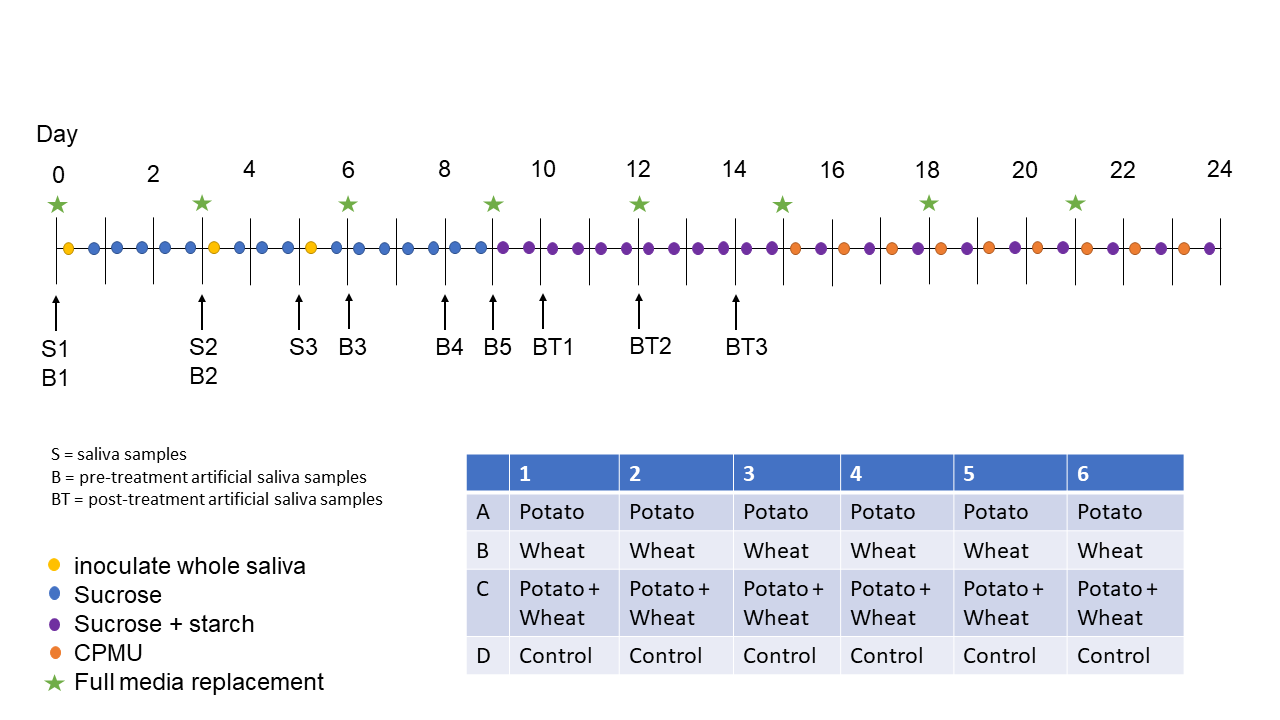
\includegraphics[width=0.7\linewidth]{../figures/protocol_overview} 

}

\caption{Overview of experiment protocol including the plate setup.}\label{fig:protocol-fig}
\end{figure}

\begin{figure}[H]

{\centering 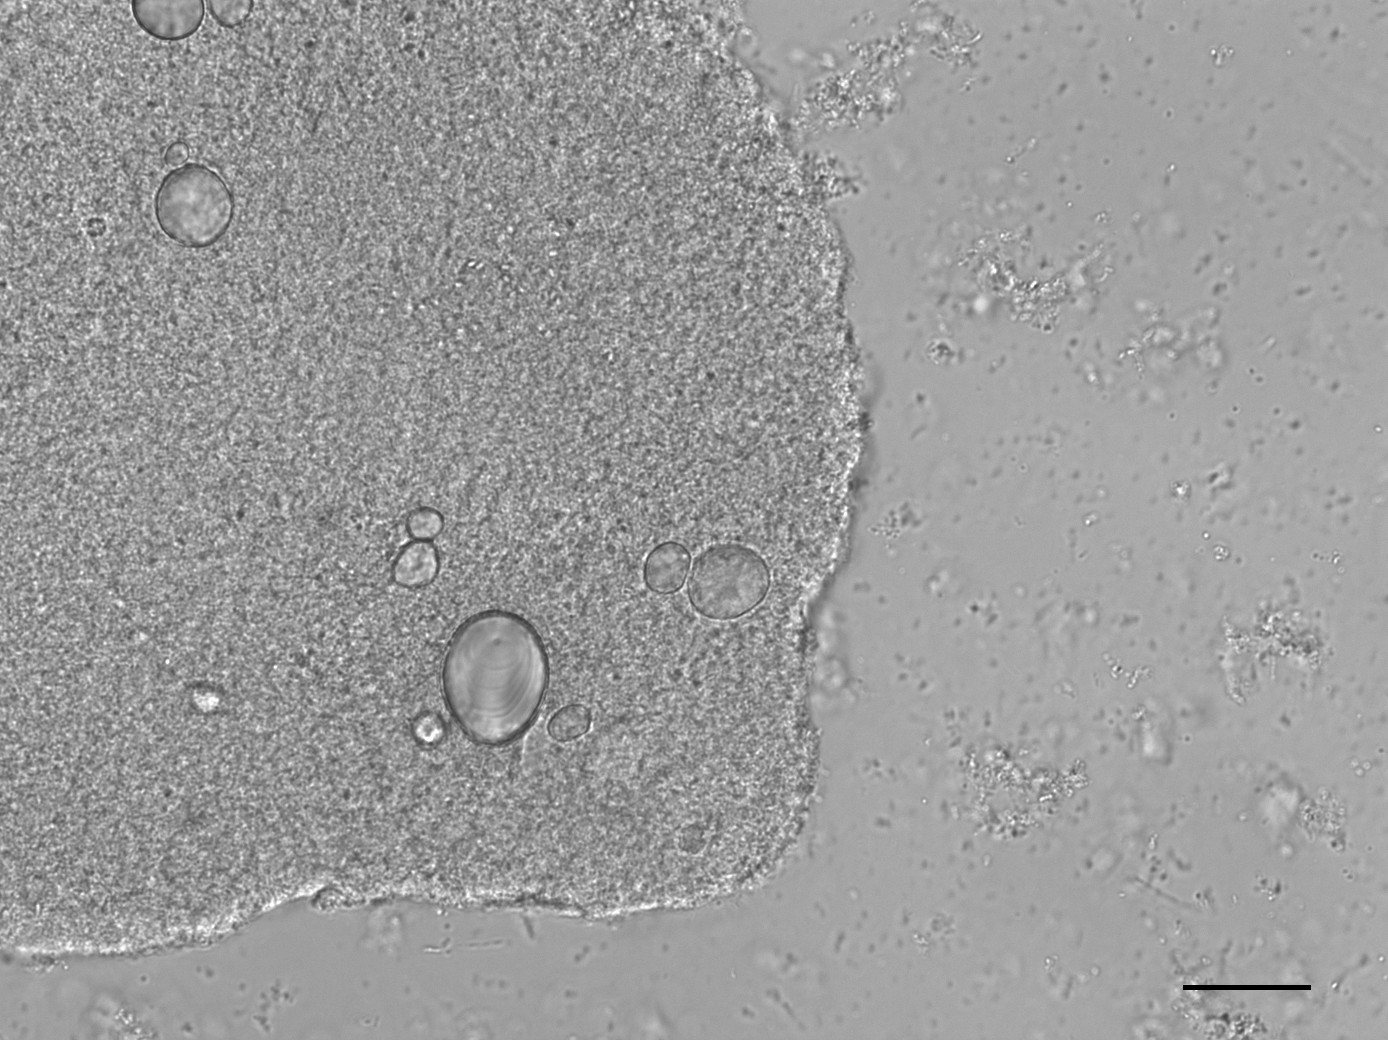
\includegraphics[width=0.4\linewidth]{../figures/starches_w_bar} 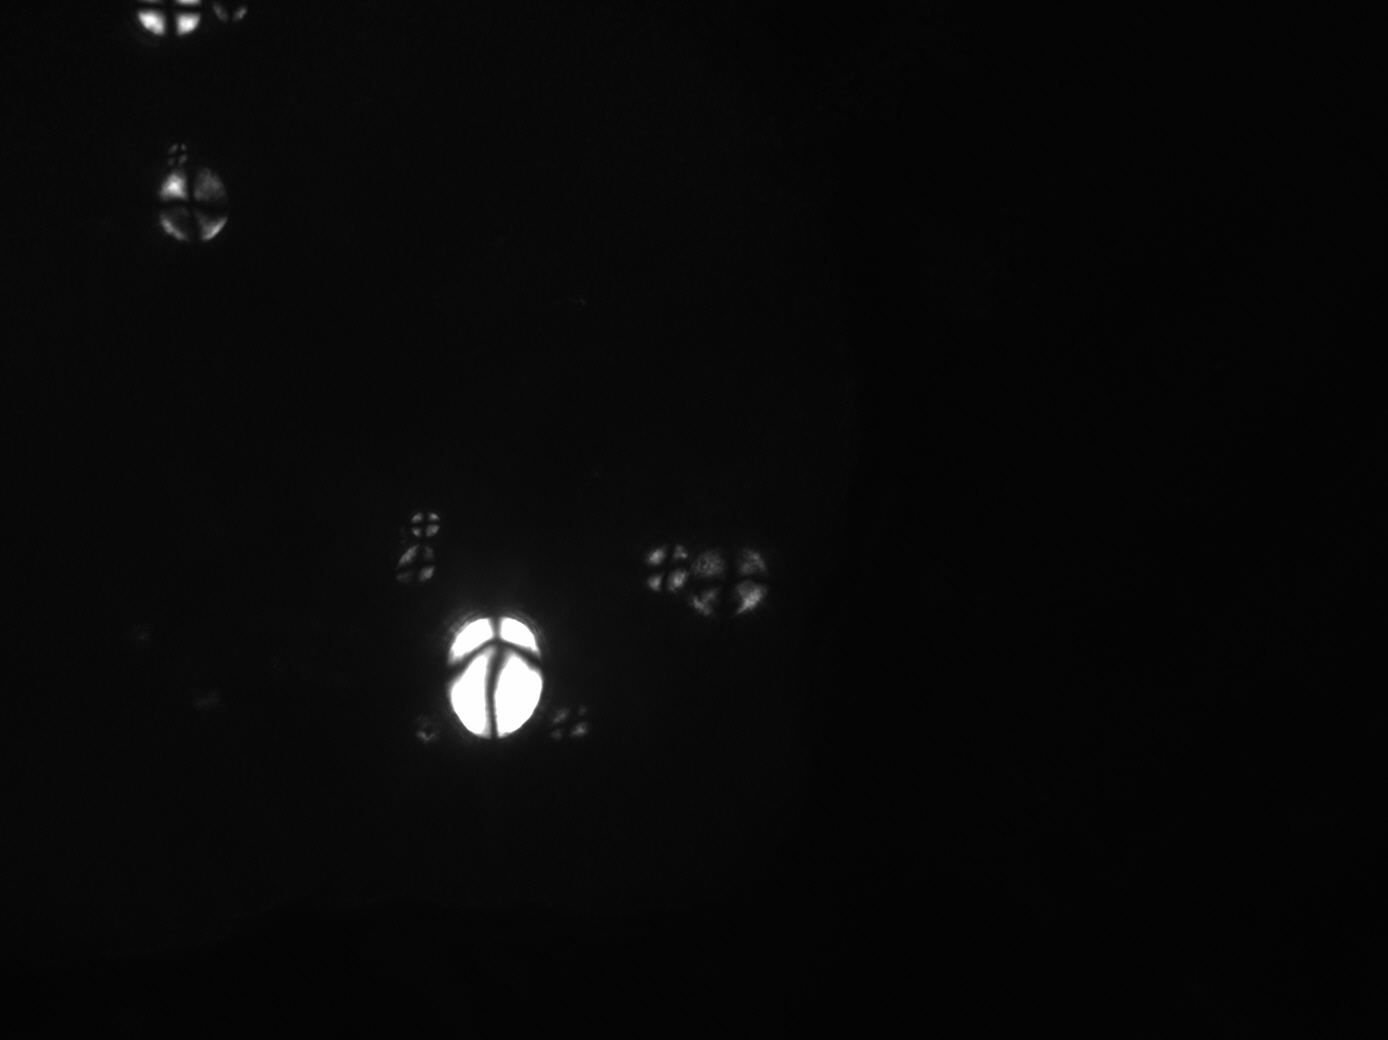
\includegraphics[width=0.4\linewidth]{../figures/st2C3.2-mix} 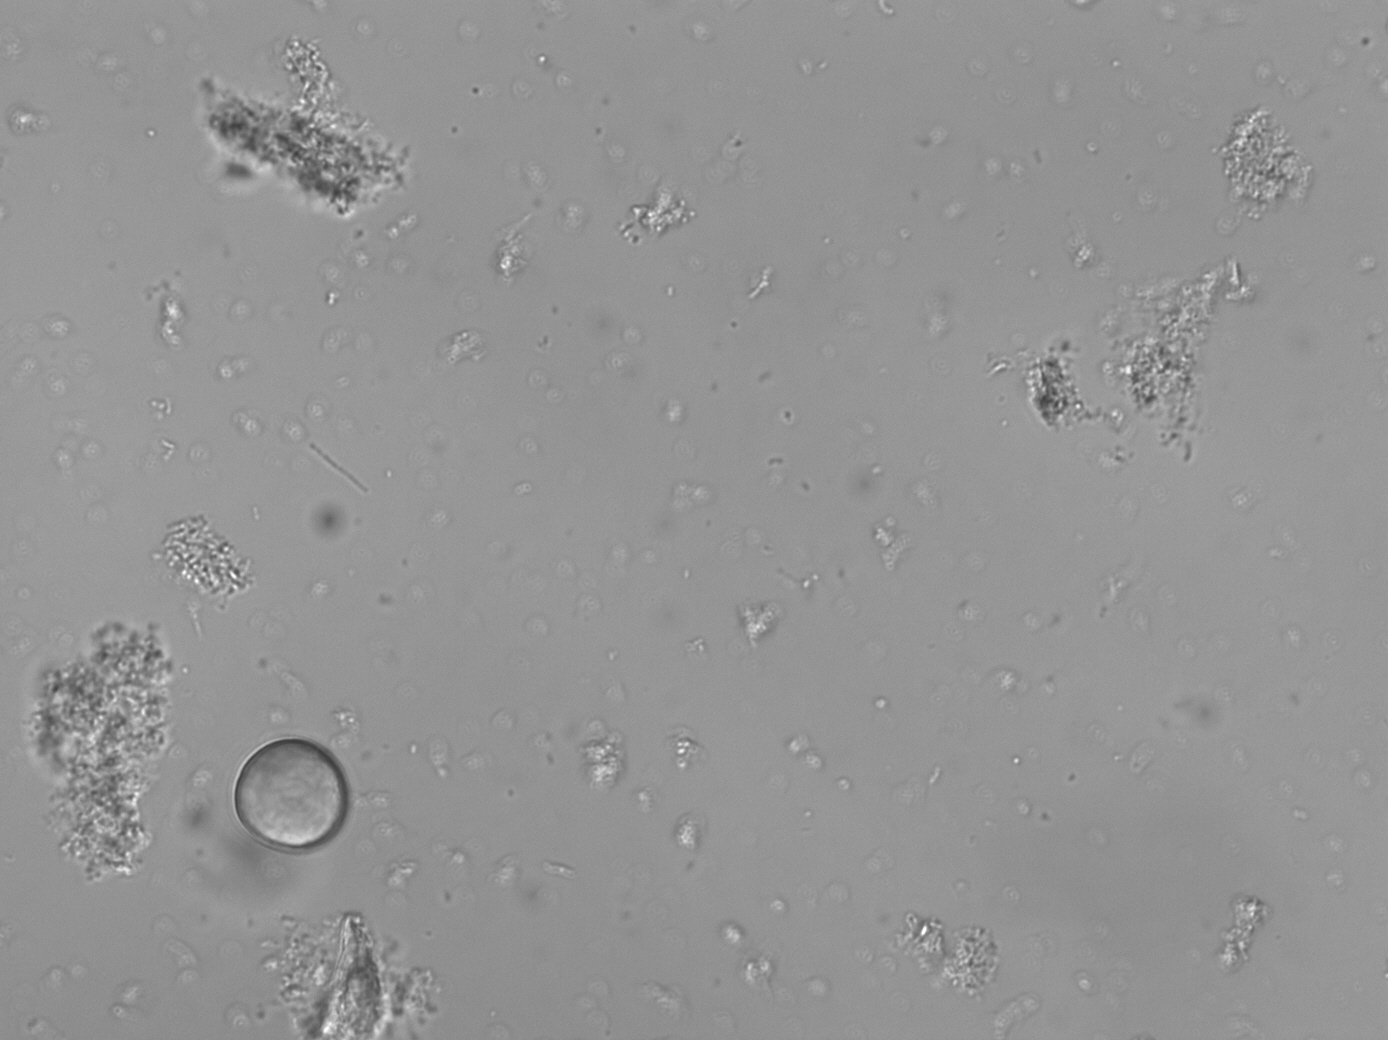
\includegraphics[width=0.4\linewidth]{../figures/st1B4-wheat} 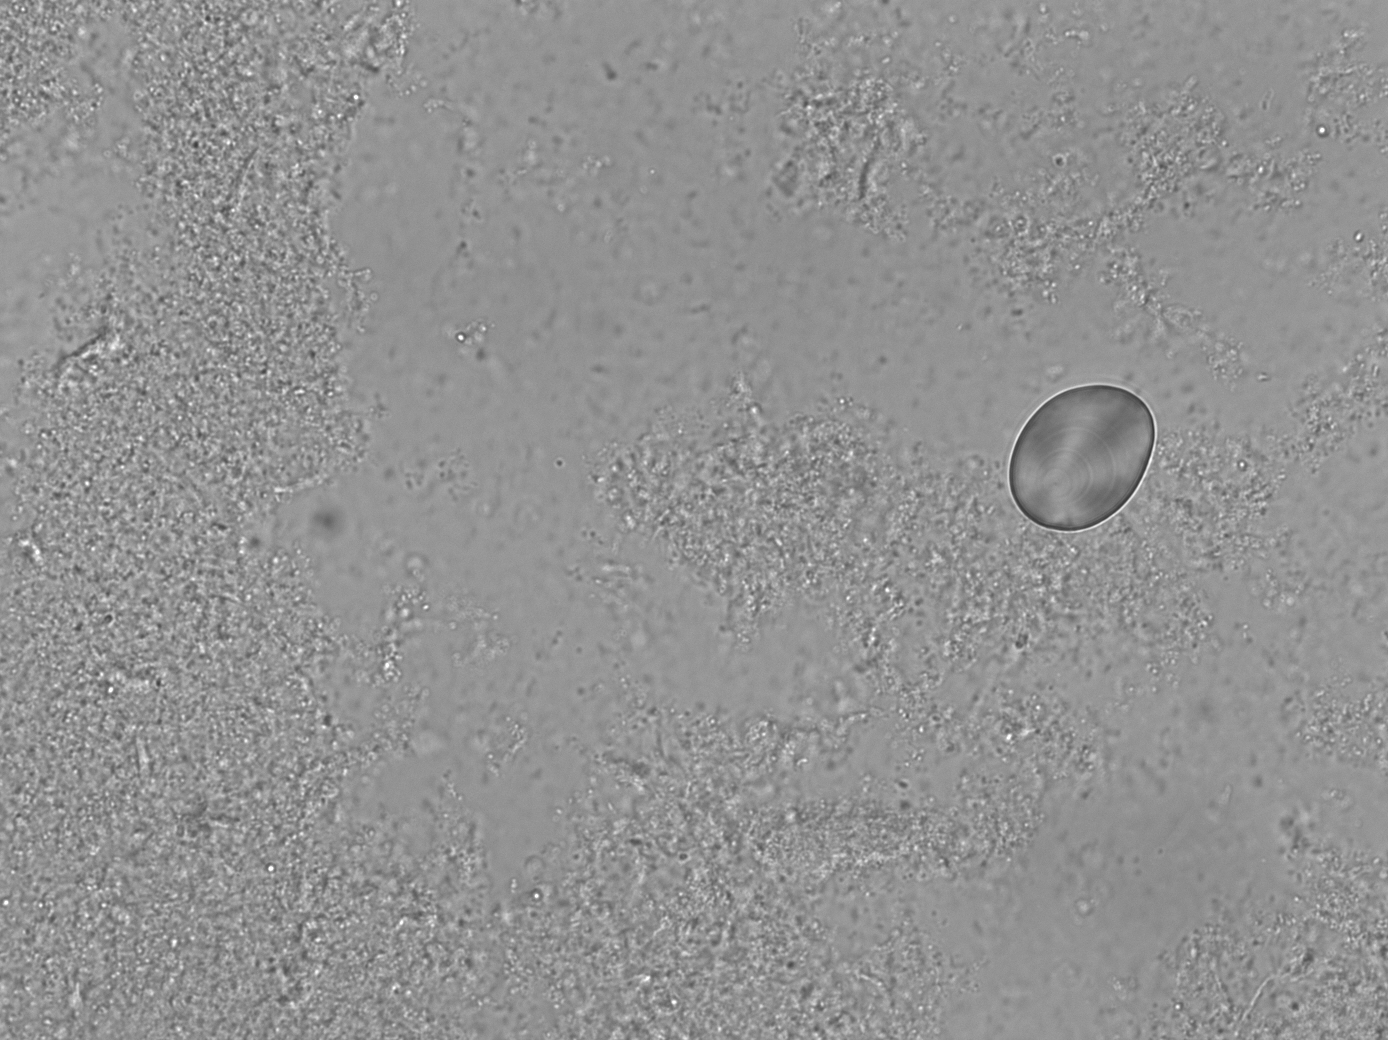
\includegraphics[width=0.4\linewidth]{../figures/2D2-potato} 

}

\caption{Microscope images of biofilm samples that were exposed to the starch solutions. Starch granules can be seen within bacterial communities and isolated. Scale bar = 20 $\mu$m.}\label{fig:microscope-fig}
\end{figure}

\begin{figure}[H]

{\centering 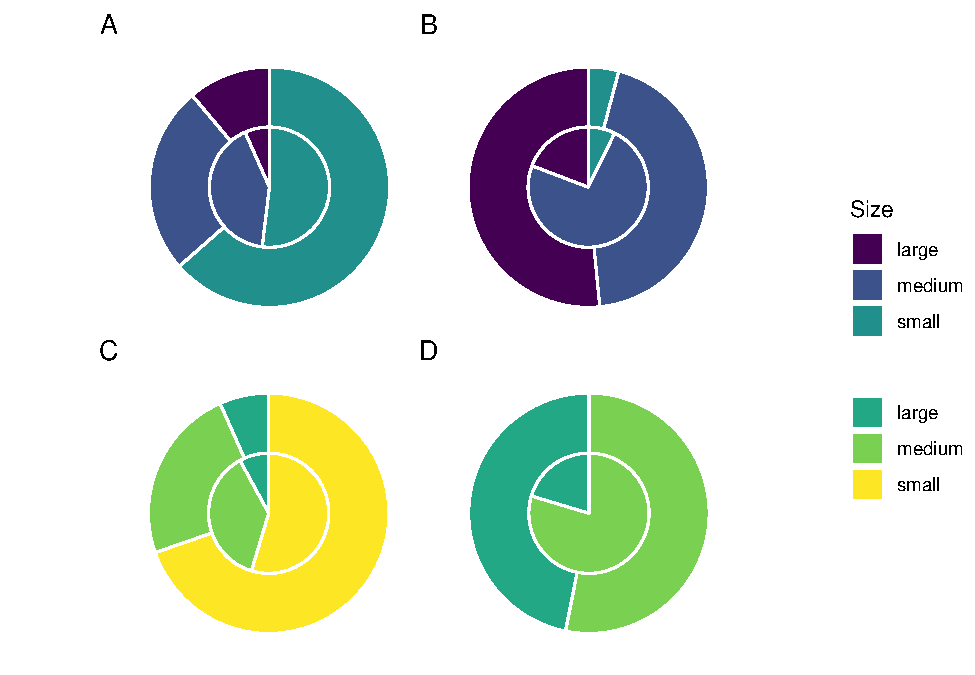
\includegraphics{../figures/ratio-plots-1} 

}

\caption{Proportion of sizes of starch granules from solutions (outer ring) and treatment samples (inner ring) in separated wheat (A) and potato (B) treatments, and mixed wheat (C) and potato (D) treatments.}\label{fig:ratio-plots}
\end{figure}

\begin{figure}[H]

{\centering 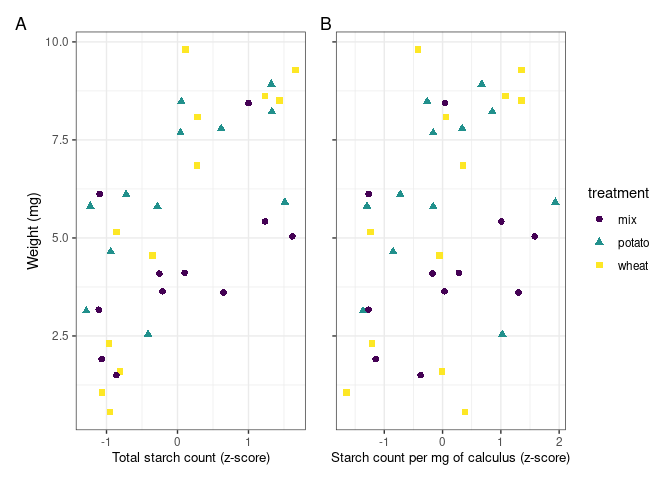
\includegraphics{../figures/cor-plot-1} 

}

\caption{Scatter plots of (A) sample weight in mg and standardised starch count by z-score for separated treatments, and (B) sample weight in mg and standardised count of starch grains per mg calculus.}\label{fig:cor-plot}
\end{figure}


\end{document}
